\documentclass[]{elsarticle} %review=doublespace preprint=single 5p=2 column
%%% Begin My package additions %%%%%%%%%%%%%%%%%%%
\usepackage[hyphens]{url}

  \journal{Landscape and Urban Planning} % Sets Journal name


\usepackage{lineno} % add
  \linenumbers % turns line numbering on
\providecommand{\tightlist}{%
  \setlength{\itemsep}{0pt}\setlength{\parskip}{0pt}}

\usepackage{graphicx}
\usepackage{booktabs} % book-quality tables
%%%%%%%%%%%%%%%% end my additions to header

\usepackage[T1]{fontenc}
\usepackage{lmodern}
\usepackage{amssymb,amsmath}
\usepackage{ifxetex,ifluatex}
\usepackage{fixltx2e} % provides \textsubscript
% use upquote if available, for straight quotes in verbatim environments
\IfFileExists{upquote.sty}{\usepackage{upquote}}{}
\ifnum 0\ifxetex 1\fi\ifluatex 1\fi=0 % if pdftex
  \usepackage[utf8]{inputenc}
\else % if luatex or xelatex
  \usepackage{fontspec}
  \ifxetex
    \usepackage{xltxtra,xunicode}
  \fi
  \defaultfontfeatures{Mapping=tex-text,Scale=MatchLowercase}
  \newcommand{\euro}{€}
\fi
% use microtype if available
\IfFileExists{microtype.sty}{\usepackage{microtype}}{}
\bibliographystyle{elsarticle-harv}
\ifxetex
  \usepackage[setpagesize=false, % page size defined by xetex
              unicode=false, % unicode breaks when used with xetex
              xetex]{hyperref}
\else
  \usepackage[unicode=true]{hyperref}
\fi
\hypersetup{breaklinks=true,
            bookmarks=true,
            pdfauthor={},
            pdftitle={Population density and the spread of the COVID-19 pandemic: a reproducible research example},
            colorlinks=false,
            urlcolor=blue,
            linkcolor=magenta,
            pdfborder={0 0 0}}
\urlstyle{same}  % don't use monospace font for urls

\setcounter{secnumdepth}{0}
% Pandoc toggle for numbering sections (defaults to be off)
\setcounter{secnumdepth}{0}

% Pandoc citation processing
\newlength{\csllabelwidth}
\setlength{\csllabelwidth}{3em}
\newlength{\cslhangindent}
\setlength{\cslhangindent}{1.5em}
% for Pandoc 2.8 to 2.10.1
\newenvironment{cslreferences}%
  {}%
  {\par}
% For Pandoc 2.11+
\newenvironment{CSLReferences}[3] % #1 hanging-ident, #2 entry spacing
 {% don't indent paragraphs
  \setlength{\parindent}{0pt}
  % turn on hanging indent if param 1 is 1
  \ifodd #1 \everypar{\setlength{\hangindent}{\cslhangindent}}\ignorespaces\fi
  % set entry spacing
  \ifnum #2 > 0
  \setlength{\parskip}{#2\baselineskip}
  \fi
 }%
 {}
\usepackage{calc} % for calculating minipage widths
\newcommand{\CSLBlock}[1]{#1\hfill\break}
\newcommand{\CSLLeftMargin}[1]{\parbox[t]{\csllabelwidth}{#1}}
\newcommand{\CSLRightInline}[1]{\parbox[t]{\linewidth - \csllabelwidth}{#1}}
\newcommand{\CSLIndent}[1]{\hspace{\cslhangindent}#1}

% Pandoc header
\usepackage{setspace}\doublespacing
\usepackage{booktabs}
\usepackage{longtable}
\usepackage{array}
\usepackage{multirow}
\usepackage{wrapfig}
\usepackage{float}
\usepackage{colortbl}
\usepackage{pdflscape}
\usepackage{tabu}
\usepackage{threeparttable}
\usepackage{threeparttablex}
\usepackage[normalem]{ulem}
\usepackage{makecell}
\usepackage{xcolor}



\begin{document}
\begin{frontmatter}

  \title{Population density and the spread of the COVID-19 pandemic: a
reproducible research example}
    \author[University]{Author\corref{1}}
   \ead{author@institution.edu} 
      \address[University]{Department, Street, City, State ZIP}
      \cortext[1]{Corresponding Author}
  
  \begin{abstract}
  The emergence of the novel SARS-CoV-2 coronavirus and the global
  COVID-19 pandemic has led to explosive growth in scientific research.
  Of interest has been the associations between population density and
  the spread of the pandemic. In this paper, population density and the
  basic reproductive number of SARS-CoV-2 are examined in an example of
  reproducible research. Given the high stakes of the situation, it is
  essential that scientific activities, on which good policy depends,
  are as transparent and reproducible as possible. Reproducibility is
  key for the efficient operation of the self-correction mechanisms of
  science. Transparency and openness means that the same problem can,
  with relatively modest efforts, be examined by independent researchers
  who can verify findings, and bring to bear different perspectives,
  approaches, and methods---sometimes with consequential changes in the
  conclusions, as the empirical example of the spread of COVID-19 in the
  US shows.
  \end{abstract}
  
 \end{frontmatter}

\newpage

\hypertarget{introduction}{%
\section{Introduction}\label{introduction}}

The emergence of the novel SARS-CoV-2 coronavirus in 2019, and the
global pandemic that followed in its wake, led to an explosive growth of
research around the globe. According to Fraser et al. (2021), over
125,000 COVID-19-related papers were released in the first ten months
from the first confirmed case of the disease. Of these, more than 30,000
were shared in pre-print servers, the use of which also exploded in the
past year (Añazco et al., 2021; Kwon, 2020; Vlasschaert et al., 2020).

Given the heavy human and economic cost of the pandemic, there has been
a natural tension in the scientific community between the need to
publish research results quickly and the imperative to maintain
consistently high quality standards in scientific reporting; indeed, a
call for maintaining the standards in published research has termed this
deluge of publications a ``carnage of substandard research'' (Bramstedt,
2020). Part of the challenge of maintaining quality standards in
published research is that, despite an abundance of recommendations and
guidelines (Broggini et al., 2017; Brunsdon and Comber, 2020; Ince et
al., 2012; Ioannidis et al., 2014), in practice reproducibility has
remained a lofty and somewhat aspirational goal (Konkol et al., 2019;
Konkol and Kray, 2019). As reported in the literature, only a woefully
small proportion of published research was actually reproducible before
the pandemic (Iqbal et al., 2016; Stodden et al., 2018), and the
situation does not appear to have changed substantially since (Gustot,
2020; Sumner et al., 2020).

The push for open data and software, along with more strenuous efforts
towards open, reproducible research, is simply a continuation of
long-standing scientific practices of independent verification. Despite
the (at times disproportionate) attention that high profile scandals in
science tend to elicit in the media, science as a collective endeavor is
remarkable for being a self-correcting enterprise, one with built-in
mechanisms and incentives to weed out erroneous ideas. Over the long
term, facts tend to prevail in science. At stake is the shorter-term
impacts that research may have in other spheres of economic and social
life. The case of economists Reinhart and Rogoff comes to mind: by the
time the inaccuracies and errors in their research were uncovered (see
Herndon et al., 2014), their claims about debt and economic growth had
already been seized by policy-makers on both sides of the Atlantic to
justify austerity policies in the aftermath of the Great Recession of
2007-2009\footnote{Nobel Prize in Economics Paul Krugman noted that
  ``Reinhart--Rogoff may have had more immediate influence on public
  debate than any previous paper in the history of economics''
  \url{https://www.nybooks.com/articles/2013/06/06/how-case-austerity-has-crumbled/?pagination=false}}.
As later research has demonstrated, those policies cast a long shadow,
and their sequels continued to be felt for years (Basu et al., 2017).

In the context of COVID-19, a topic that has grabbed the imagination of
numerous thinkers has been the prospect of life in cities after the
pandemic (Florida et al., 2020); the implications are the topic of
ongoing research (Sharifi and Khavarian-Garmsir, 2020). The fact that
the worst of the pandemic was initially felt in dense population centers
such as Wuhan, Milan, Madrid, and New York, brought a torrent of
research into the associations between density and the spread of the
pandemic. Some important questions hang on the results of these research
efforts. For example, are lower density regions safer from the pandemic?
Are de-densification policies warranted, even if just in the short term?
And in the longer term, will the risks of life in high density regions
presage a flight from cities? What are the implications of the pandemic
for future urban planning and practice? Over the past year, numerous
papers have sought to throw light into the underlying issue of density
and the pandemic; nonetheless the results, as will be detailed next,
remain mixed. Further, to complicate matters, precious few of these
studies appear to be sufficiently open to support independent
verification.

The objective of this paper is to illustrate the importance of
reproducibility in research in the context of the flood of COVID-19
papers. To this end, a recent study by Sy et al. (2021) is chosen as an
example of reproducible research. The objective is not to malign the
analysis of these researchers, but rather to demonstrate the value of
openness to allow for independent verification and further analysis.
Open data and open code mean that an independent researcher can, with
only modest efforts, not only verify the findings reported, but also
examine the same data from a perspective which may not have been
available to the original researchers due to differences in disciplinary
perspectives, methodological traditions, and/or training, among other
possible factors. The example, which shows consequential changes in the
conclusions reached by different analyses, should serve as a call to
researchers to redouble their efforts to increase transparency and
reproducibility in research. This paper, in addition, aims to show how
data can be packaged in well-documented, shareable units, and code can
be embedded into self-contained documents suitable for review and
independent verification. The source for this paper is an
\href{http://rmarkdown.rstudio.com}{R Markdown} document which, along
with the data package, will be available in a public
repository\footnote{For peer-review purposes, the data package and code
  are currently in an anonymous Drive folder:
  \url{https://drive.google.com/drive/folders/1cT6tcUc1pJ4aT5ajQ0emO0lyS46P8Ige?usp=sharing}}.

\hypertarget{background-the-intuitive-relationship-between-density-and-spread-of-contagious-diseases}{%
\section{Background: the intuitive relationship between density and
spread of contagious
diseases}\label{background-the-intuitive-relationship-between-density-and-spread-of-contagious-diseases}}

The concern with population density and the spread of the virus during
the COVID-19 pandemic was fueled, at least in part, by dramatic scenes
seen in real-time around the world from large urban centers such as
Wuhan, Milan, Madrid, and New York. In theory, there are good reasons to
believe that higher density may have a positive association with the
transmission of a contagious virus. It has long been known that the
potential for inter-personal contact is greater in regions with higher
density (see for example the research on urban fields and
time-geography, including Farber and Páez, 2011; Moore, 1970; Moore and
Brown, 1970). Mathematically, models of exposure and contagion indicate
that higher densities can catalyze the transmission of contagious
diseases (Li et al., 2018; Rocklöv and Sjödin, 2020). The idea is
intuitive and likely at the root of messages, by some figures in
positions of authority, that regions with sparse population densities
faced lower risks from the pandemic\footnote{Governor Kristi Noem of
  South Dakota, for example, claimed that sparse population density
  allowed her state to face the pandemic down without the need for
  strict policy interventions
  \url{https://www.inforum.com/lifestyle/health/5025620-South-Dakota-is-not-New-York-City-Noem-defends-lack-of-statewide-COVID-19-restrictions}}.

As Rocklöv and Sjödin (Rocklöv and Sjödin, 2020) note, however,
mathematical models of contagion are valid at small-to-medium spatial
scales (and presumably, small temporal scales too, such as time spent in
restaurants, concert halls, cruises), and the results do not necessarily
transfer to larger spatial units and different time scales. There are
solid reasons for this: while in a restaurant, one can hardly avoid
being in proximity to other customers-however, a person can choose to
(or be forced to as a matter of policy) not go to a restaurant in the
first place. Nonetheless, the idea that high density correlates with
high transmission is so seemingly reasonable that it is often taken for
granted even at larger scales (e.g., Cruz et al., 2020; Micallef et al.,
2020). At larger scales, however, there exists the possibility of
behavioral adaptations, which are difficult to capture in the
mechanistic framework of differential equations (or can be missing in
agent-based models, e.g., Gomez et al., 2021); these adaptations, in
fact, can be a key aspect of disease transmission.

A plausible behavioral adaptation during a pandemic, especially one
broadcast as widely and intensely as COVID-19, is risk compensation.
Risk compensation is a process whereby people adjust their behavior in
response to their \emph{perception} of risk (Noland, 1995; Phillips et
al., 2011; Richens et al., 2000). In the case of COVID-19, Chauhan et
al. (Chauhan et al., 2021) have found that perception of risks in the US
varies between rural, suburban, and urban residents, with rural
residents in general expressing less concern about the virus. It is
possible that people who listened to the message of leaders saying that
they were safe because of low density may not have taken adequate
precautions against the virus. People in dense places who could more
directly observe the impact of the pandemic may have become overly
cautious. Both Paez et al. (2020) and Hamidi et al. (2020b) posit this
mechanism (i.e., greater compliance with social distancing in denser
regions) to explain the results of their analyses. The evidence
available does indeed show that there were important changes in behavior
with respect to mobility during the pandemic (Harris and Branion-Calles,
2021; Jamal and Paez, 2020; Molloy et al., 2020); furthermore, shelter
in place orders may have had greater buy-in from the public in higher
density regions (Feyman et al., 2020; Hamidi and Zandiatashbar, 2021),
and the associated behavior may have persisted beyond the duration of
official social-distancing policies (Praharaj et al., 2020). In
addition, there is evidence that changes in mobility correlated with the
trajectory of the pandemic (Noland, 2021; Paez, 2020). Given the
potential for behavioral adaptation, the question of density becomes
more nuanced: it is not just a matter of proximity, but also of human
behavior, which is better studied using population-level data and
models.

\hypertarget{background-but-what-does-the-literature-say}{%
\section{Background: but what does the literature
say?}\label{background-but-what-does-the-literature-say}}

When it comes to population density and the spread of COVID-19, the
international literature to date remains inconclusive.

On the one hand, there are studies that report positive associations
between population density and various COVID-19-related outcomes. Bhadra
(2021), for example, reported a moderate positive correlation between
the spread of COVID-19 and population density at the district level in
India, however their analysis was bivariate and did not control for
other variables, such as income. Similarly, Kadi and Khelfaoui (2020)
found a positive and significant correlation between number of cases and
population density in cities in Algeria in a series of simple regression
models (i.e., without other controls). A question in these relatively
simple analyses is whether density is not a proxy for other factors.
Other studies have included controls, such as Pequeno et al. (2020), a
team that reported a positive association between density and cumulative
counts of confirmed COVID-19 cases in state capitals in Brazil after
controlling for covariates, including income, transport connectivity,
and economic status. In a similar vein, Fielding-Miller et al. (2020)
reported a positive relationship between the absolute number of COVID-19
deaths and population density (rate) in rural counties in the US. Roy
and Ghosh (2020) used a battery of machine learning techniques to find
discriminatory factors, and a positive and significant association
between COVID-19 infection and death rates in US states. Wong and Li
(2020) also found a positive and significant association between
population density and number of confirmed COVID-19 cases in US
counties, using both univariate and multivariate regressions with
spatial effects. More recently, Sy et al. (2021) reported that the basic
reproductive number of COVID-19 in US counties tended to increase with
population density, but at a decreasing rate at higher densities.

On the flip side, a number of studies report non-significant or negative
associations between population density and COVID-19 outcomes. This
includes the research of Sun et al. (2020) who did not find evidence of
significant correlation between population density and confirmed number
of cases per day \emph{in conditions of lockdown} in China. This finding
echoes the results of Paez et al. (2020), who in their study of
provinces in Spain reported non-significant associations between
population density and infection rates in the early days of the first
wave of COVID-19, and negative significant associations in the later
part of the first lockdown. Similarly, (2020) found zero or negative
associations between population density and infection numbers/deaths by
country. Fielding-Miller et al. (2020) contrast their finding about
rural counties with a negative relationship between COVID-19 deaths and
population density in urban counties in the US. For their part, in their
investigation of doubling time, White and Hébert-Dufresne (2020)
identified a negative and significant correlation between population
density and doubling time in US states. Likewise, (2021) fond a small
negative (and significant) association between population density and
COVID-19 morbidity in districts in Tehran. Finally, two of the most
complete studies in the US {[}by Hamidi et al.; (2020a); (2020b){]} used
an extensive set of controls to find negative and significant
correlations between density and COVID-19 cases and fatalities at the
level of counties in the US.

As can be seen, these studies are implemented at different scales in
different regions of the world. They also use a range of techniques,
from correlation analysis, to multivariate regression, spatial
regressions, and machine learning techniques. This is natural and to be
expected: individual researchers have only limited time and expertise.
This is why reproducibility is important. To pick an example (which will
be further elaborated in later sections of this paper), the study of Sy
et al.~{[}(2021); hereafter SWN{]} would immediately grab the attention
of a researcher with a somewhat different toolbox.

\hypertarget{reproducibility-of-research}{%
\section{Reproducibility of
research}\label{reproducibility-of-research}}

SWN investigated the basic reproductive number of COVID-19 in US
counties, and its association with population density, median household
income, and prevalence of private mobility. For their multivariate
analysis, SWN used mixed linear models. This is a reasonable modelling
choice: \(R_0\) is an interval-ratio variable that is suitably modeled
using linear regression; further, as SWN note there is a likelihood that
the process in not independent ``among counties within each state,
potentially due to variable resource allocation and differing health
systems across states'' (p.~3). A mixed linear model accounts for this
by introducing random components (in the case of SWN, random intercepts
at the state level). SWN estimated various models with different
combinations of variables, including median household income and
prevalence of travel by private transportation. These are sensible
controls, given potential variations in behavior: people in more
affluent counties may have greater opportunities to work from home, and
use of private transportation reduces contact with strangers. Moreover,
they also conducted various sensitivity analyses. After these efforts,
SWN conclude that there is a positive association between the basic
reproductive number and population density at the level of counties in
the US.

One salient aspect of the analysis in SWN is that the basic reproductive
number can only be calculated reliably with a minimum number of cases,
and a large number of counties did not meet such threshold. As
researchers do, SWN made modelling decisions, in this case basing their
analysis only on counties with valid observations. A modeler with
expertise in different methods would likely ask some of the following
questions on reading SWN's paper: how were missing counties treated?
What are the implications of the spatial sampling framework used in the
analysis? Is it possible to spatially interpolate the missing
observations? These questions are relevant and their implications
important. Fortunately, SWN are an example of a reasonably open,
reproducible research product: their paper is accompanied by (most of)
the data and (most of) the code used in the analysis. This means that an
independent expert can, with only a moderate investment of time and
effort, reproduce the results in the paper, as well as ask additional
questions.

Alas, reproducibility is not necessarily the norm in the relevant
literature.

There are various reasons why a project can fail to be reproducible. In
some cases, there might be legitimate reasons to withhold the data,
perhaps due to confidentiality and privacy reasons (e.g., Lee et al.,
2020). But in many other cases the data are publicly available, which in
fact has commonly been the case with population-level COVID-19
information. Typically the provenance of the data is documented, but in
numerous studies the data themselves are not shared (Amadu et al., 2021;
Bhadra et al., 2021; Cruz et al., 2020; Feng et al., 2020;
Fielding-Miller et al., 2020; Hamidi et al., 2020a, 2020b; Inbaraj et
al., 2021; Souris and Gonzalez, 2020). As any researcher can attest,
whether a graduate student or a seasoned scientist, collecting,
organizing, and preparing data for a project can take a substantial
amount of time. Pointing to the sources of data, even when these sources
are public, is a small step towards reproducibility-but only a very
small one. Faced with the prospect of having to recreate a data set from
raw sources is probably sufficient to dissuade all but the most
dedicated (or stubborn) researcher from independent verification. This
is true even if part of the data are shared (e.g., Wong and Li, 2020).
In other cases, data are shared, but the processes followed in the
preparation of the data are not fully documented (Ahmad et al., 2020;
Skórka et al., 2020). These processes matter, as shown by the errors in
the spreadsheets of Reinhart and Rogoff (Herndon et al., 2014) and the
data of biologist Jonathan Pruitt that led to an ``avalanche'' of paper
retractions\footnote{\url{https://doi.org/10.1038/d41586-020-00287-y}}.
Another situation is when papers share well-documented data, but fail to
provide the code used in the analysis (Noury et al., 2021; Pequeno et
al., 2020; Wang et al., 2021). Making code available only ``on demand''
(e.g., Brandtner et al., 2021) is an unnecessary barrier when most
journals offer the facility to share supplemental materials online. Then
there are those papers that more closely comply with reproducibility
standards, and share well-documented processes and data, as well as the
code used in any analyses reported (Feyman et al., 2020; Paez et al.,
2020; Stephens et al., 2021; Sy et al., 2021; White and Hébert-Dufresne,
2020).

In the following sections, the analysis of RWN is reproduced, some
relevant questions from the perspective of an independent researcher are
asked, and the data are reanalyzed.

\hypertarget{reproducing-swn}{%
\section{Reproducing SWN}\label{reproducing-swn}}

SWN examined the association between the basic reproductive number of
COVID-19 and population density. The basic reproductive number \(R_0\)
is a summary measure of contact rates, probability of transmission of a
pathogen, and duration of infectiousness. In rough terms, \(R_0\)
measures how many new infections each infections begets. Infectious
disease outbreaks generally tend to die out when \(R_0<1\), and to grow
when \(R_0>1\). Reliable calculation of \(R_0\) requires a minimum
number of cases to be able to assume that there is community
transmission of the pathogen. Accordingly, SWN based their analysis only
on counties that had at least 25 cases or more at the end of the
exponential growth phase (see Fig. \ref{fig:R0-map}). Their final sample
included 1,151 counties in the US, including in Alaska, Hawaii, Puerto
Rico, and island territories.

\begin{figure}
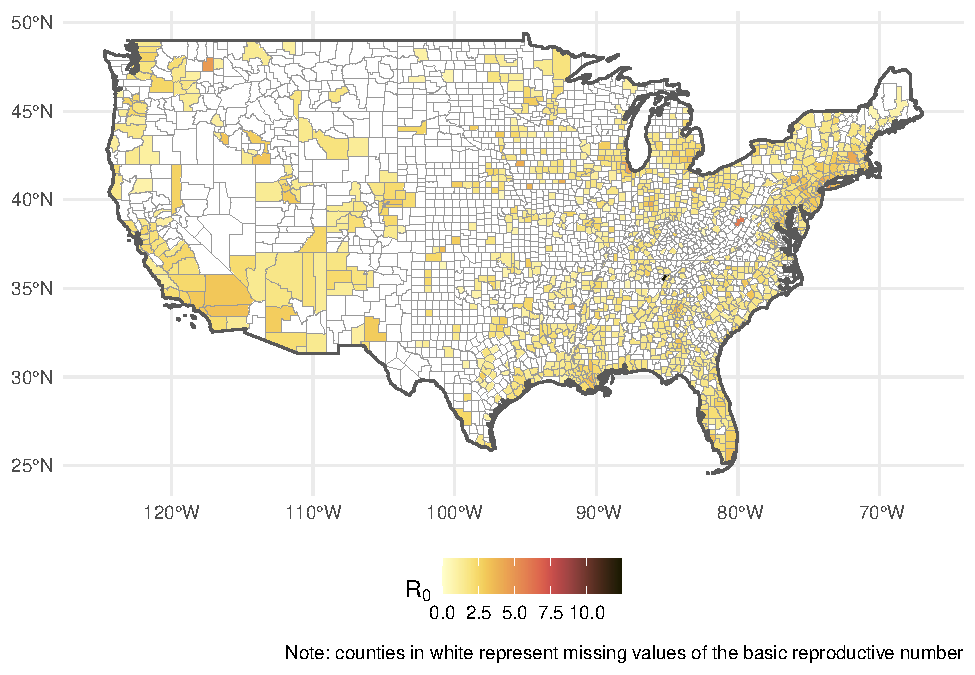
\includegraphics[width=1\linewidth]{R0-Density-Reanalysis_files/figure-latex/R0-map-1} \caption{\label{fig:R0-map}Basic reproductive rate in US counties (Alaska, Hawaii, Puerto Rico, and territories not shown).}\label{fig:R0-map}
\end{figure}

Table \ref{tab:swn-results} reproduces the first three models of SWN
(the fourth model did not have any significant variables; see Table 1 in
SWN). It is possible to verify that the results match, with only the
minor (and irrelevant) exception of the magnitude of the coefficient for
travel by private transportation, which is due to a difference in the
input (here the variable is one percent units, whereas in SWN it was ten
percent units). The mixed linear model gives random intercepts (i.e.,
the intercept is a random variable), and the standard deviation is
reported in the fourth row of Table \ref{tab:swn-results}. It is useful
to map the random intercepts: as seen in Figure
\ref{fig:random-terms-map}, other things being equal, counties in Texas
tend to have somewhat lower values of \(R_0\) (i.e., a negative random
intercept), whereas counties in South Dakota tend to have higher values
of \(R_0\). The key of the analysis, after extensive sensitivity
analysis, is a robust finding that population density has a positive
association with the basic reproductive number. But does it?

\begin{table}

\caption{\label{tab:tabulate-swn-results}\label{tab:swn-results}Reproducing SWN: Models 1-3}
\centering
\resizebox{\linewidth}{!}{
\begin{tabular}[t]{lllllrl}
\toprule
\multicolumn{1}{c}{ } & \multicolumn{2}{c}{Model 1} & \multicolumn{2}{c}{Model 2} & \multicolumn{2}{c}{Model 3} \\
\cmidrule(l{3pt}r{3pt}){2-3} \cmidrule(l{3pt}r{3pt}){4-5} \cmidrule(l{3pt}r{3pt}){6-7}
Variable & beta & 95\% CI & beta & 95\% CI & beta & 95\% CI\\
\midrule
Intercept & 2.274 & [2.167, 2.381] & 3.347 & [2.676, 4.018] & 3.386 & [2.614, 4.157]\\
Log of population density & 0.162 & [0.133, 0.191] & 0.145 & [0.115, 0.176] & 0.147 & [0.113, 0.18]\\
Percent of private transportation &  &  & -0.013 & [-0.02, -0.005] & -0.013 & [-0.021, -0.005]\\
Median household income (\$10,000) &  &  &  &  & -0.003 & [-0.033, 0.026]\\
Standard deviation (Intercept) & 0.166 & [0.108, 0.254] & 0.136 & [0.081, 0.229] & 0.137 & [0.081, 0.232]\\
\addlinespace
Within-group standard error & 0.665 & [0.638, 0.693] & 0.665 & [0.638, 0.693] & 0.665 & [0.638, 0.694]\\
\bottomrule
\end{tabular}}
\end{table}

\begin{figure}
\includegraphics[width=1\linewidth]{R0-Density-Reanalysis_files/figure-latex/random-terms-map-1} \caption{\label{fig:random-terms-map}Random intercepts of Model 3 (Alaska, Hawaii, Puerto Rico, and territories not shown).}\label{fig:random-terms-map}
\end{figure}

\hypertarget{expanding-on-swn}{%
\section{Expanding on SWN}\label{expanding-on-swn}}

The preceding section shows that thanks to the availability of code and
data, it is possible to verify the results reported by SWN. As noted
earlier, though, an independent researcher might have wondered about the
implications of the spatial sampling procedure used by SWN. The decision
to use a sample of counties with reliable basic reproductive numbers,
although apparently sensible, results in a non-random spatial sampling
scheme. Turning our attention back to Figure \ref{fig:R0-map}, we form
the impression that many counties without reliable values of \(R_0\) are
in more rural, less dense parts of the United States. This impression is
reinforced when we overlay the boundaries of urban areas with population
greater than 50,000 on the counties with valid values of \(R_0\) (see
Figure \ref{fig:urban-areas-map}). The fact that \(R_0\) could not be
accurately computed in many counties without large urban areas does not
mean that there was no transmission of the virus: it simply means that
we do not know with precision whether that was the case. The low number
of cases may be related to low population and/or low population density.
This is intriguing, to say the least: by excluding cases based on the
ability to calculate \(R_0\) we are potentially \emph{censoring} the
sample in a non-random way.

\begin{figure}
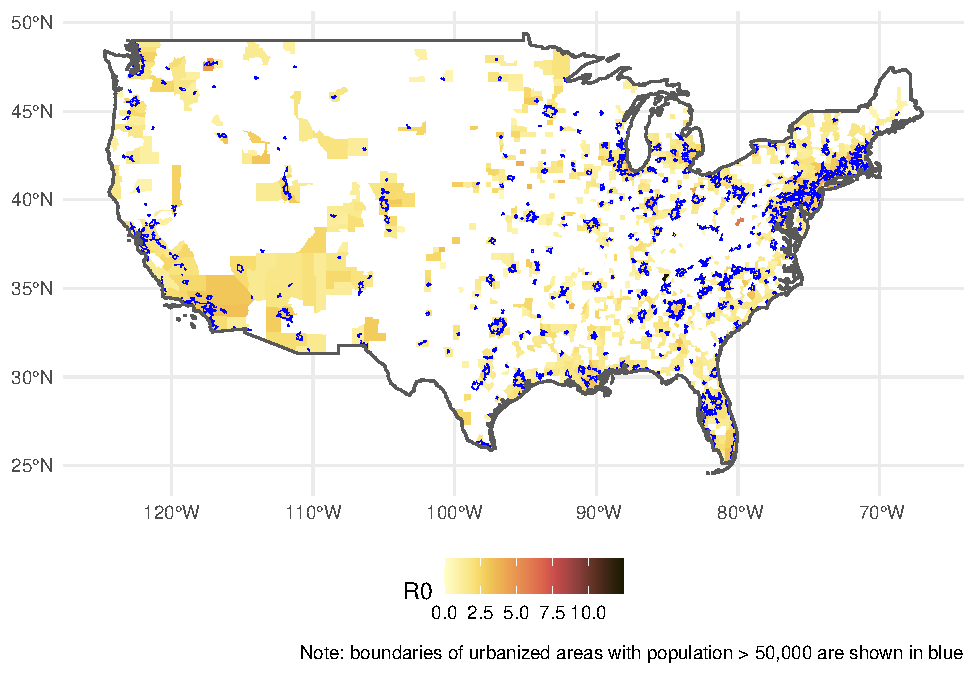
\includegraphics[width=1\linewidth]{R0-Density-Reanalysis_files/figure-latex/urban-areas-map-1} \caption{\label{fig:urban-areas-map}Urban areas with population > 50,000 (Alaska, Hawaii, Puerto Rico, and territories not shown).}\label{fig:urban-areas-map}
\end{figure}

A problematic issue with non-random sample selection is that parameter
estimates can become unreliable, and numerous techniques have been
developed over time to address this. A model useful for sample selection
problems is Heckman's selection model (see Maddala, 1983). The selection
model is in fact a system of two equations, as follows:

\[
\begin{array}{c}
y_i^{S*} = \beta^{S\prime}x_i^S+\epsilon_i^S\\
y_i^{O*} = \beta^{O\prime}x_i^O+\epsilon_i^O
\end{array}
\] \noindent where \(y_i^{S*}\) is a latent variable for the sample
selection process, and \(y_i^{O*}\) is the latent outcome. Vectors
\(x_i^S\) and \(x_i^O\) are explanatory variables (with the possibility
that \(x_i^S = x_i^S\)). Both equations include random terms (i.e.,
\(\epsilon_i^S\) and \(\epsilon_i^O\)) The first equation is designed to
model the \emph{probability} of sampling, and the second equation the
outcome of interest (say \(R_0\)). The random terms are jointly
distributed and correlated with parameter \(\rho\).

What the analyst observes is the following: \[
y_i^S =
\begin{cases}
0 & \text{if } y_i^{S*} < 0\\
1 & \text{otherwise}
\end{cases}
\] \noindent and: \[
y_i^O =
\begin{cases}
0 & \text{if } y_i^{S} = 0\\
y_i^{O*} & \text{otherwise}
\end{cases}
\]

In other words, the outcome of interest is observed \emph{only} for
certain cases (\(y_i^S=1\), i.e., for sampled observations). The
probability of sampling depends on \(x_i^S\). For the cases observed,
the outcome \(y_i^O\) depends on \(x_i^O\).

A sample selection model is estimated using the same selection of
variables as SWN Model 3. This is Sample Selection Model 1 in Table
\ref{tab:selection-results}. The first thing to notice about this model
is that the sample selection process and the outcome are not independent
(\(\rho\ne0\) with 5\% of confidence). The selection equation indicates
that the probability of a county to be in the sample increases with
population density (but at a decreasing rate due to the
log-transformation), when travel by private modes is more prevalent, and
as median household income in the county is higher. This is in line with
the impression left by Figure \ref{fig:urban-areas-map} that counties
with reliable values of \(R_0\) tended to be those with larger urban
centers. Once that the selection probabilities are accounted for in the
model, several things happen with the outcomes model. First, the
coefficient for population density is still positive, but the magnitude
changes: in effect, it appears that the effect of density is more
pronounced than what SWN Model 3 indicated. The coefficient for percent
of private transportation changes signs. And the coefficient for median
household income is now significant.

The second model in Table \ref{tab:selection-results} (Selection Model
2) changes the way the variables are entered into the model. The
log-transformation of density in SWN and Selection Model 1 assumes that
the association between density and \(R_0\) is monotonically increasing
(if the sign of the coefficient is positive) or decreasing (if the sign
of the coefficient is negative). There are some indications that the
relationship may actually not be monotonical. For example, Paez et al.
(2020) found a positive (if non-significant) relationship between
density and incidence of COVID-19 in the provinces of Spain at the
beginning of the pandemic. This changed to a negative (and significant)
relationship during the lockdown. In the case of the US, Fielding-Miller
et al. (2020) found that the association between COVID-19 deaths and
population density was positive in rural counties, but negative in urban
counties. A variable transformation that allows for non-monotonic
changes in the relationship is the square of the density.

As seen in the table, Selection Model 2 replaces the log-transformation
of population density with a quadratic expansion. The results of this
analysis indicate that with this variable transformation, the selection
and outcome processes are still not independent (\(\rho\ne0\) with 5\%
of confidence). But a few interesting things emerge. When we examine the
outcomes model, we see that the quadratic expansion has a positive
coefficient for the first order term, but a negative coefficient for the
second order term. This indicates that \(R_0\) initially tends to
increase with higher density, but only up to a point, after which the
negative second term (which grows more rapidly due to the square),
becomes increasingly dominant. Secondly, the sign of the coefficient for
travel by private transportation becomes negative again. This, of
course, makes more sense than the positive sign of Selection Model 1: if
people tend to travel in private transportation, the potential for
contact should be lower instead of higher. And finally median household
income is no longer significant.

\begin{table}

\caption{\label{tab:tabulate-sample-selection-results}\label{tab:selection-results}Estimation results of sample selection models}
\centering
\resizebox{\linewidth}{!}{
\begin{tabular}[t]{lcccc}
\toprule
\multicolumn{1}{c}{ } & \multicolumn{2}{c}{Selection Model 1} & \multicolumn{2}{c}{Selection Model 2} \\
\cmidrule(l{3pt}r{3pt}){2-3} \cmidrule(l{3pt}r{3pt}){4-5}
Variable & $\beta$ & 95\% CI & $\beta$ & 95\% CI\\
\midrule
\addlinespace[0.3em]
\multicolumn{5}{l}{\textbf{Sample Selection Model}}\\
\hspace{1em}Intercept & -2.237 & [-3.109, -1.365] & -7.339 & [-8.381, -6.297]\\
\hspace{1em}Log of population density & 0.385 & [0.352, 0.418] &  & \\
\hspace{1em}Density (1,000 per sq.km) &  &  & 2.484 & [2.13, 2.838]\\
\hspace{1em}Density squared &  &  & -0.387 & [-0.473, -0.3]\\
\hspace{1em}Percent of private transportation & 0.025 & [0.016, 0.034] & 0.057 & [0.046, 0.067]\\
\hspace{1em}Median household income (10,000) & 0.202 & [0.168, 0.235] & 0.32 & [0.283, 0.357]\\
\addlinespace[0.3em]
\multicolumn{5}{l}{\textbf{Outcome Model}}\\
\hspace{1em}Intercept & 0.605 & [-0.257, 1.466] & 2.784 & [1.652, 3.915]\\
\hspace{1em}Log of population density & 0.39 & [0.354, 0.426] &  & \\
\hspace{1em}Density (1,000 per sq.km) &  &  & 0.758 & [0.509, 1.008]\\
\hspace{1em}Density squared &  &  & -0.132 & [-0.187, -0.077]\\
\hspace{1em}Percent of private transportation & 0.01 & [0.001, 0.018] & -0.011 & [-0.021, -0.001]\\
\hspace{1em}Median household income (\$10,000) & 0.126 & [0.094, 0.159] & 0.002 & [-0.033, 0.037]\\
$\sigma$ & 0.954 & [0.904, 1.003] & 0.684 & [0.652, 0.716]\\
$\rho$ & 0.971 & [0.961, 0.98] & -0.199 & [-0.377, -0.022]\\
\bottomrule
\end{tabular}}
\end{table}

How relevant is the difference between these different model
specifications? Figure \ref{fig:comparison-results} shows the
relationship between density and \(R_0\) implied by SWN Model 1 and
Selection Model 2. The left panel of the figure shows the non-linear but
monotonic relationship implied by SWN Model 1. The conclusion is that at
higher densities, \(R_0\) is \emph{always} higher. The right panel, in
contrast, shows that, according to Selection Model 2, \(R_0\) is zero
when density is zero (as expected), and then it tends to increase at
higher densities. This continues until a density of approximately 2.9
(1,000 people per sq.km). At higher densities than that \(R_0\) begins
to decline, and the relationship becomes negative at densities higher
than approximately 5.7 (1,000 people per sq.km).

Thus, other things being equal, the effect of density in a county like
Charlottesville in Virginia (density \textasciitilde1,639 people per
sq.km) is roughly the same as that in a county like Philadelphia
(density \textasciitilde4,127 people per sq.km). In contrast, the effect
of density on \(R_0\) in a county like Arlington in Virginia (density
\textasciitilde3,093 people per sq.km) is \emph{stronger} than either of
the previous two examples. Lastly, the density of counties like San
Francisco in California, or Queens and Bronx in NY, which are among the
densest in the US, contributes even less to \(R_0\) than even the most
rural counties in the country.

It is worth at this point to recall Cressie's dictum about modelling:
``{[}w{]}hat is one person's mean structure could be another person's
correlation structure'' (Cressie, 1989, p. 201). There are almost always
multiple ways to approach a modelling situation. In the present case, we
would argue that spatial sampling is an important aspect of the modeling
process, but one that perhaps required different technical skills than
those available to SWN. There is nothing wrong with that. What matters
is that, by adopting relatively high reproducibility standards, these
researchers made a valuable and honest contribution to the collective
enterprise of seeking knowledge. Their effort, and subsequent efforts to
validate and expand on their work, can potentially contribute to provide
clarity to ongoing conversations about the relevance of density and the
spread of COVID-19.

In particular, it is noteworthy that a sample selection model with a
different variable transformation does not lend support to the thesis
that higher density is \emph{always} associated with a greater risk of
spread of the virus {[}as put by Wong and Li, ``\,`Density is destiny'
is probably an overstatement''; (2020){]}. At the same time, this also
stands in contrast to the findings of Hamidi et al., who found that
higher density was either not significantly associated with the rate of
the virus in a cross-sectional study (Hamidi et al., 2020b), or was
negatively associated with in a longitudinal setting {[}Hamidi et al.
(2020a). In this sense, the conclusion that density does not aggravate
the pandemic may have been somewhat premature; instead, reanalysis of
the data of SWN suggests that Fielding-Miller et al. (2020) might be
onto something with respect to the difference between rural and urban
counties. More generally, in population-level studies, density is
indicative of proximity, no doubt about that, but also for adaptive
behavior. And it is possible that the determining factor during
COVID-19, at least in the US, has been variations in perceptions of the
risks associated with contagion (Chauhan et al., 2021), and subsequent
compensations in behavior in more and less dense regions.

\begin{figure}
\includegraphics[width=1\linewidth]{R0-Density-Reanalysis_files/figure-latex/comparison-results-1} \caption{\label{fig:comparison-results}Effect of density according to SWN Model 3 and Sample Selection Model 2.}\label{fig:comparison-results}
\end{figure}

\hypertarget{conclusion}{%
\section{Conclusion}\label{conclusion}}

The tension between the need to publish research potentially useful in
dealing with a global pandemic, and a ``carnage of substandard
research'' (Bramstedt, 2020), highlights the importance of efforts to
maintain the quality of scientific outputs during COVID-19. An important
part of quality control is the ability of independent researchers to
verify and examine the results of materials published in the literature.
As previous research illustrates, reproducibility in scientific research
remains an important but elusive goal (Gustot, 2020; e.g., Iqbal et al.,
2016; Stodden et al., 2018; Sumner et al., 2020). This idea is
reinforced by the review conducted for this paper in the context of
research about population density and the spread of COVID-19.

Taking one recent example from the literature {[}Sy et al., Sy et al.
(2021); SWN{]}, the present paper illustrates the importance of good
reproducibility practices. Sharing data and code can catalyze research,
by allowing independent verification of findings, as well as additional
research. After verifying the results of SWN, experiments with sample
selection models and variations in the definition of model inputs, lead
to an important reappraisal of the conclusion that high density is
associated with greater spread of the virus. Instead, the possibility of
a non-monotonical relationship between population density and contagion
is raised.

In the spirit of openness, this paper is prepared as an R Markdown
document, an a companion data package is provided. The data package
contains the relevant documentation of the data, and all data
pre-processing is fully documented. Hopefully this, and similar
reproducible papers, will continue to encourage others to adopt
reproducible standards in their research.

\hypertarget{references}{%
\section*{References}\label{references}}
\addcontentsline{toc}{section}{References}

\hypertarget{refs}{}
\begin{CSLReferences}{1}{0}
\leavevmode\hypertarget{ref-Ahmad2020association}{}%
Ahmad, K., Erqou, S., Shah, N., Nazir, U., Morrison, A.R., Choudhary,
G., Wu, W.-C., 2020. Association of poor housing conditions with
COVID-19 incidence and mortality across US counties. PLOS ONE 15,
e0241327.
doi:\href{https://doi.org/10.1371/journal.pone.0241327}{10.1371/journal.pone.0241327}

\leavevmode\hypertarget{ref-Amadu2021assessing}{}%
Amadu, I., Ahinkorah, B.O., Afitiri, A.-R., Seidu, A.-A., Ameyaw, E.K.,
Hagan, J.E., Duku, E., Aram, S.A., 2021. Assessing sub-regional-specific
strengths of healthcare systems associated with COVID-19 prevalence,
deaths and recoveries in africa. PLOS ONE 16, e0247274.
doi:\href{https://doi.org/10.1371/journal.pone.0247274}{10.1371/journal.pone.0247274}

\leavevmode\hypertarget{ref-Anazco2021publication}{}%
Añazco, D., Nicolalde, B., Espinosa, I., Camacho, J., Mushtaq, M.,
Gimenez, J., Teran, E., 2021. Publication rate and citation counts for
preprints released during the COVID-19 pandemic: The good, the bad and
the ugly. PeerJ 9, e10927.
doi:\href{https://doi.org/10.7717/peerj.10927}{10.7717/peerj.10927}

\leavevmode\hypertarget{ref-Basu2017ten}{}%
Basu, S., Carney, M.A., Kenworthy, N.J., 2017. Ten years after the
financial crisis: The long reach of austerity and its global impacts on
health. Social Science \& Medicine 187, 203--207.
doi:\href{https://doi.org/10.1016/j.socscimed.2017.06.026}{10.1016/j.socscimed.2017.06.026}

\leavevmode\hypertarget{ref-Bhadra2021impact}{}%
Bhadra, A., Mukherjee, A., Sarkar, K., 2021. Impact of population
density on covid-19 infected and mortality rate in india. Modeling Earth
Systems and Environment 7, 623--629.
doi:\href{https://doi.org/10.1007/s40808-020-00984-7}{10.1007/s40808-020-00984-7}

\leavevmode\hypertarget{ref-Bramstedt2020carnage}{}%
Bramstedt, K.A., 2020. The carnage of substandard research during the
COVID-19 pandemic: A call for quality. Journal of Medical Ethics 46,
803--807.
doi:\href{https://doi.org/10.1136/medethics-2020-106494}{10.1136/medethics-2020-106494}

\leavevmode\hypertarget{ref-Brandtner2021creatures}{}%
Brandtner, C., Bettencourt, L.M.A., Berman, M.G., Stier, A.J., 2021.
Creatures of the state? Metropolitan counties compensated for state
inaction in initial u.s. Response to COVID-19 pandemic. PLOS ONE 16,
e0246249.
doi:\href{https://doi.org/10.1371/journal.pone.0246249}{10.1371/journal.pone.0246249}

\leavevmode\hypertarget{ref-Broggini2017reproducible}{}%
Broggini, F., Dellinger, J., Fomel, S., Liu, Y., 2017. Reproducible
research: Geophysics papers of the future - introduction. Geophysics 82.
doi:\href{https://doi.org/10.1190/geo2017-0918-spseintro.1}{10.1190/geo2017-0918-spseintro.1}

\leavevmode\hypertarget{ref-Brunsdon2020opening}{}%
Brunsdon, C., Comber, A., 2020. Opening practice: Supporting
reproducibility and critical spatial data science. Journal of
Geographical Systems.
doi:\href{https://doi.org/10.1007/s10109-020-00334-2}{10.1007/s10109-020-00334-2}

\leavevmode\hypertarget{ref-Chauhan2021covid}{}%
Chauhan, R.S., Capasso da Silva, D., Salon, D., Shamshiripour, A.,
Rahimi, E., Sutradhar, U., Khoeini, S., Mohammadian, A.(Kouros).,
Derrible, S., Pendyala, R., 2021. COVID-19 related attitudes and risk
perceptions across urban, rural, and suburban areas in the united
states. Findings.
doi:\href{https://doi.org/10.32866/001c.23714}{10.32866/001c.23714}

\leavevmode\hypertarget{ref-Cressie1989geostatistics}{}%
Cressie, N., 1989. Geostatistics. The American Statistician 43, 197.
doi:\href{https://doi.org/10.2307/2685361}{10.2307/2685361}

\leavevmode\hypertarget{ref-Cruz2020exploring}{}%
Cruz, C.J.P., Ganly, R., Li, Z., Gietel-Basten, S., 2020. Exploring the
young demographic profile of COVID-19 cases in hong kong: Evidence from
migration and travel history data. PLOS ONE 15, e0235306.
doi:\href{https://doi.org/10.1371/journal.pone.0235306}{10.1371/journal.pone.0235306}

\leavevmode\hypertarget{ref-Farber2011running}{}%
Farber, S., Páez, A., 2011. Running to stay in place: The time-use
implications of automobile oriented land-use and travel. Journal of
Transport Geography 19, 782--793.
doi:\href{https://doi.org/10.1016/j.jtrangeo.2010.09.008}{10.1016/j.jtrangeo.2010.09.008}

\leavevmode\hypertarget{ref-Feng2020spread}{}%
Feng, Y., Li, Q., Tong, X., Wang, R., Zhai, S., Gao, C., Lei, Z., Chen,
S., Zhou, Y., Wang, J., Yan, X., Xie, H., Chen, P., Liu, S., Xv, X.,
Liu, S., Jin, Y., Wang, C., Hong, Z., Luan, K., Wei, C., Xu, J., Jiang,
H., Xiao, C., Guo, Y., 2020. Spatiotemporal spread pattern of the
COVID-19 cases in china. PLOS ONE 15, e0244351.
doi:\href{https://doi.org/10.1371/journal.pone.0244351}{10.1371/journal.pone.0244351}

\leavevmode\hypertarget{ref-Feyman2020effectiveness}{}%
Feyman, Y., Bor, J., Raifman, J., Griffith, K.N., 2020. Effectiveness of
COVID-19 shelter-in-place orders varied by state. PLOS ONE 15, e0245008.
doi:\href{https://doi.org/10.1371/journal.pone.0245008}{10.1371/journal.pone.0245008}

\leavevmode\hypertarget{ref-Fielding2020social}{}%
Fielding-Miller, R.K., Sundaram, M.E., Brouwer, K., 2020. Social
determinants of COVID-19 mortality at the county level. PLOS ONE 15,
e0240151.
doi:\href{https://doi.org/10.1371/journal.pone.0240151}{10.1371/journal.pone.0240151}

\leavevmode\hypertarget{ref-Florida2020how}{}%
Florida, R., Glaeser, E., Sharif, M., Bedi, K., Campanella, T., Chee,
C., Doctoroff, D., Katz, B., Katz, R., Kotkin, J., 2020. How life in our
cities will look after the coronavirus pandemic. Foreign Policy 1.

\leavevmode\hypertarget{ref-Fraser2021evolving}{}%
Fraser, N., Brierley, L., Dey, G., Polka, J.K., Pálfy, M., Nanni, F.,
Coates, J.A., 2021. The evolving role of preprints in the dissemination
of COVID-19 research and their impact on the science communication
landscape. PLOS Biology 19, e3000959.
doi:\href{https://doi.org/10.1371/journal.pbio.3000959}{10.1371/journal.pbio.3000959}

\leavevmode\hypertarget{ref-Gomez2021infekta}{}%
Gomez, J., Prieto, J., Leon, E., Rodríguez, A., 2021. INFEKTA---an
agent-based model for transmission of infectious diseases: The COVID-19
case in bogotá, colombia. PLOS ONE 16, e0245787.
doi:\href{https://doi.org/10.1371/journal.pone.0245787}{10.1371/journal.pone.0245787}

\leavevmode\hypertarget{ref-Gustot2020quality}{}%
Gustot, T., 2020. Quality and reproducibility during the COVID-19
pandemic. JHEP Rep 2, 100141.
doi:\href{https://doi.org/10.1016/j.jhepr.2020.100141}{10.1016/j.jhepr.2020.100141}

\leavevmode\hypertarget{ref-Hamidi2020longitudinal}{}%
Hamidi, S., Ewing, R., Sabouri, S., 2020a. Longitudinal analyses of the
relationship between development density and the COVID-19 morbidity and
mortality rates: Early evidence from 1,165 metropolitan counties in the
united states. Health \& Place 64, 102378.
doi:\href{https://doi.org/10.1016/j.healthplace.2020.102378}{10.1016/j.healthplace.2020.102378}

\leavevmode\hypertarget{ref-Hamidi2020density}{}%
Hamidi, S., Sabouri, S., Ewing, R., 2020b. Does density aggravate the
COVID-19 pandemic? Journal of the American Planning Association 86,
495--509.
doi:\href{https://doi.org/10.1080/01944363.2020.1777891}{10.1080/01944363.2020.1777891}

\leavevmode\hypertarget{ref-Hamidi2021compact}{}%
Hamidi, S., Zandiatashbar, A., 2021. Compact development and adherence
to stay-at-home order during the COVID-19 pandemic: A longitudinal
investigation in the united states. Landscape and Urban Planning 205,
103952. doi:\url{https://doi.org/10.1016/j.landurbplan.2020.103952}

\leavevmode\hypertarget{ref-Harris2021Changes}{}%
Harris, M.A., Branion-Calles, M., 2021. Changes in commute mode
attributed to COVID-19 risk in canadian national survey data. Findings.
doi:\href{https://doi.org/10.32866/001c.19088}{10.32866/001c.19088}

\leavevmode\hypertarget{ref-Herndon2014high}{}%
Herndon, T., Ash, M., Pollin, R., 2014. Does high public debt
consistently stifle economic growth? A critique of reinhart and rogoff.
Cambridge Journal of Economics 38, 257--279.
doi:\href{https://doi.org/10.1093/cje/bet075}{10.1093/cje/bet075}

\leavevmode\hypertarget{ref-Inbaraj2021seroprevalence}{}%
Inbaraj, L.R., George, C.E., Chandrasingh, S., 2021. Seroprevalence of
COVID-19 infection in a rural district of south india: A
population-based seroepidemiological study. PLOS ONE 16, e0249247.
doi:\href{https://doi.org/10.1371/journal.pone.0249247}{10.1371/journal.pone.0249247}

\leavevmode\hypertarget{ref-Ince2012case}{}%
Ince, D.C., Hatton, L., Graham-Cumming, J., 2012. The case for open
computer programs. Nature 482, 485--488.
doi:\href{https://doi.org/10.1038/nature10836}{10.1038/nature10836}

\leavevmode\hypertarget{ref-Ioannidis2014increasing}{}%
Ioannidis, J.P.A., Greenland, S., Hlatky, M.A., Khoury, M.J., Macleod,
M.R., Moher, D., Schulz, K.F., Tibshirani, R., 2014. Increasing value
and reducing waste in research design, conduct, and analysis. Lancet
383, 166--175.
doi:\href{https://doi.org/10.1016/s0140-6736(13)62227-8}{10.1016/s0140-6736(13)62227-8}

\leavevmode\hypertarget{ref-Iqbal2016reproducible}{}%
Iqbal, S.A., Wallach, J.D., Khoury, M.J., Schully, S.D., Ioannidis,
J.P.A., 2016. Reproducible research practices and transparency across
the biomedical literature. Plos Biology 14.
doi:\href{https://doi.org/10.1371/journal.pbio.1002333}{10.1371/journal.pbio.1002333}

\leavevmode\hypertarget{ref-Jamal2020Changes}{}%
Jamal, S., Paez, A., 2020. Changes in trip-making frequency by mode
during COVID-19. Findings.
doi:\href{https://doi.org/10.32866/001c.17977}{10.32866/001c.17977}

\leavevmode\hypertarget{ref-Kadi2020population}{}%
Kadi, N., Khelfaoui, M., 2020. Population density, a factor in the
spread of COVID-19 in algeria: Statistic study. Bulletin of the National
Research Centre 44.
doi:\href{https://doi.org/10.1186/s42269-020-00393-x}{10.1186/s42269-020-00393-x}

\leavevmode\hypertarget{ref-Khavarian2021high}{}%
Khavarian-Garmsir, A.R., Sharifi, A., Moradpour, N., 2021. Are
high-density districts more vulnerable to the COVID-19 pandemic?
Sustainable Cities and Society 70, 102911.
doi:\href{https://doi.org/10.1016/j.scs.2021.102911}{10.1016/j.scs.2021.102911}

\leavevmode\hypertarget{ref-Konkol2019examination}{}%
Konkol, M., Kray, C., 2019. In-depth examination of spatiotemporal
figures in open reproducible research. Cartography and Geographic
Information Science 46, 412--427.
doi:\href{https://doi.org/10.1080/15230406.2018.1512421}{10.1080/15230406.2018.1512421}

\leavevmode\hypertarget{ref-Konkol2019computational}{}%
Konkol, M., Kray, C., Pfeiffer, M., 2019. Computational reproducibility
in geoscientific papers: Insights from a series of studies with
geoscientists and a reproduction study. International Journal of
Geographical Information Science 33, 408--429.
doi:\href{https://doi.org/10.1080/13658816.2018.1508687}{10.1080/13658816.2018.1508687}

\leavevmode\hypertarget{ref-Kwon2021swamped}{}%
Kwon, D., 2020. How swamped preprint servers are blocking bad
coronavirus research. Nature 581, 130--132.

\leavevmode\hypertarget{ref-Lee2020human}{}%
Lee, M., Zhao, J., Sun, Q., Pan, Y., Zhou, W., Xiong, C., Zhang, L.,
2020. Human mobility trends during the early stage of the COVID-19
pandemic in the united states. PLOS ONE 15, e0241468.
doi:\href{https://doi.org/10.1371/journal.pone.0241468}{10.1371/journal.pone.0241468}

\leavevmode\hypertarget{ref-Li2018effect}{}%
Li, R., Richmond, P., Roehner, B.M., 2018. Effect of population density
on epidemics. Physica A: Statistical Mechanics and its Applications 510,
713--724.
doi:\href{https://doi.org/10.1016/j.physa.2018.07.025}{10.1016/j.physa.2018.07.025}

\leavevmode\hypertarget{ref-Maddala1983limited}{}%
Maddala, G.S., 1983. Limited-dependent and qualitative variables in
econometrics. Cambridge University Press, Cambridge.

\leavevmode\hypertarget{ref-Micallef2020first}{}%
Micallef, S., Piscopo, T.V., Casha, R., Borg, D., Vella, C., Zammit,
M.-A., Borg, J., Mallia, D., Farrugia, J., Vella, S.M., Xerri, T.,
Portelli, A., Fenech, M., Fsadni, C., Mallia Azzopardi, C., 2020. The
first wave of COVID-19 in malta; a national cross-sectional study. PLOS
ONE 15, e0239389.
doi:\href{https://doi.org/10.1371/journal.pone.0239389}{10.1371/journal.pone.0239389}

\leavevmode\hypertarget{ref-Molloy2020Tracing}{}%
Molloy, J., Tchervenkov, C., Hintermann, B., Axhausen, K.W., 2020.
Tracing the sars-CoV-2 impact: The first month in switzerland. Findings.
doi:\href{https://doi.org/10.32866/001c.12903}{10.32866/001c.12903}

\leavevmode\hypertarget{ref-Moore1970some}{}%
Moore, E.G., 1970. Some spatial properties of urban contact fields.
Geographical Analysis 2, 376--386.

\leavevmode\hypertarget{ref-Moore1970urban}{}%
Moore, E.G., Brown, L.A., 1970. Urban acquaintance fields: An evaluation
of a spatial model. Environment and Planning 2, 443--454.

\leavevmode\hypertarget{ref-Noland1995perceived}{}%
Noland, R.B., 1995. PERCEIVED RISK AND MODAL CHOICE - RISK COMPENSATION
IN TRANSPORTATION SYSTEM. Accident Analysis and Prevention 27, 503--521.
doi:\href{https://doi.org/10.1016/0001-4575(94)00087-3}{10.1016/0001-4575(94)00087-3}

\leavevmode\hypertarget{ref-Noland2021mobility}{}%
Noland, R.B., 2021. Mobility and the effective reproduction rate of
COVID-19. Journal of Transport \& Health 20, 101016.
doi:\url{https://doi.org/10.1016/j.jth.2021.101016}

\leavevmode\hypertarget{ref-Noury2021how}{}%
Noury, A., François, A., Gergaud, O., Garel, A., 2021. How does COVID-19
affect electoral participation? Evidence from the french municipal
elections. PLOS ONE 16, e0247026.
doi:\href{https://doi.org/10.1371/journal.pone.0247026}{10.1371/journal.pone.0247026}

\leavevmode\hypertarget{ref-Paez2020using}{}%
Paez, A., 2020. Using google community mobility reports to investigate
the incidence of COVID-19 in the united states. Findings.
doi:\url{https://doi.org/10.32866/001c.12976}

\leavevmode\hypertarget{ref-Paez2020spatio}{}%
Paez, A., Lopez, F.A., Menezes, T., Cavalcanti, R., Pitta, M.G. da R.,
2020. A spatio-temporal analysis of the environmental correlates of
COVID-19 incidence in spain. Geographical Analysis n/a.
doi:\href{https://doi.org/10.1111/gean.12241}{10.1111/gean.12241}

\leavevmode\hypertarget{ref-Pequeno2020air}{}%
Pequeno, P., Mendel, B., Rosa, C., Bosholn, M., Souza, J.L., Baccaro,
F., Barbosa, R., Magnusson, W., 2020. Air transportation, population
density and temperature predict the spread of COVID-19 in brazil. PeerJ
8, e9322.
doi:\href{https://doi.org/10.7717/peerj.9322}{10.7717/peerj.9322}

\leavevmode\hypertarget{ref-Phillips2011risk}{}%
Phillips, R.O., Fyhri, A., Sagberg, F., 2011. Risk compensation and
bicycle helmets. Risk Analysis 31, 1187--1195.
doi:\href{https://doi.org/10.1111/j.1539-6924.2011.01589.x}{10.1111/j.1539-6924.2011.01589.x}

\leavevmode\hypertarget{ref-Praharaj2020Using}{}%
Praharaj, S., King, D., Pettit, C., Wentz, E., 2020. Using aggregated
mobility data to measure the effect of COVID-19 policies on mobility
changes in sydney, london, phoenix, and pune. Findings.
doi:\href{https://doi.org/10.32866/001c.17590}{10.32866/001c.17590}

\leavevmode\hypertarget{ref-Richens2000condoms}{}%
Richens, J., Imrie, J., Copas, A., 2000. Condoms and seat belts: The
parallels and the lessons. Lancet 355, 400--403.
doi:\href{https://doi.org/10.1016/s0140-6736(99)09109-6}{10.1016/s0140-6736(99)09109-6}

\leavevmode\hypertarget{ref-Rocklov2020high}{}%
Rocklöv, J., Sjödin, H., 2020. High population densities catalyse the
spread of COVID-19. Journal of Travel Medicine 27.
doi:\href{https://doi.org/10.1093/jtm/taaa038}{10.1093/jtm/taaa038}

\leavevmode\hypertarget{ref-Roy2020factors}{}%
Roy, S., Ghosh, P., 2020. Factors affecting COVID-19 infected and death
rates inform lockdown-related policymaking. PLOS ONE 15, e0241165.
doi:\href{https://doi.org/10.1371/journal.pone.0241165}{10.1371/journal.pone.0241165}

\leavevmode\hypertarget{ref-Sharifi2020covid}{}%
Sharifi, A., Khavarian-Garmsir, A.R., 2020. The COVID-19 pandemic:
Impacts on cities and major lessons for urban planning, design, and
management. Science of The Total Environment 749, 142391.
doi:\url{https://doi.org/10.1016/j.scitotenv.2020.142391}

\leavevmode\hypertarget{ref-Skorka2020macroecology}{}%
Skórka, P., Grzywacz, B., Moroń, D., Lenda, M., 2020. The macroecology
of the COVID-19 pandemic in the anthropocene. PLOS ONE 15, e0236856.
doi:\href{https://doi.org/10.1371/journal.pone.0236856}{10.1371/journal.pone.0236856}

\leavevmode\hypertarget{ref-Souris2020covid}{}%
Souris, M., Gonzalez, J.-P., 2020. COVID-19: Spatial analysis of
hospital case-fatality rate in france. PLOS ONE 15, e0243606.
doi:\href{https://doi.org/10.1371/journal.pone.0243606}{10.1371/journal.pone.0243606}

\leavevmode\hypertarget{ref-Stephens2021impact}{}%
Stephens, K.E., Chernyavskiy, P., Bruns, D.R., 2021. Impact of altitude
on COVID-19 infection and death in the united states: A modeling and
observational study. PLOS ONE 16, e0245055.
doi:\href{https://doi.org/10.1371/journal.pone.0245055}{10.1371/journal.pone.0245055}

\leavevmode\hypertarget{ref-Stodden2018empirical}{}%
Stodden, V., Seiler, J., Ma, Z.K., 2018. An empirical analysis of
journal policy effectiveness for computational reproducibility.
Proceedings of the National Academy of Sciences of the United States of
America 115, 2584--2589.
doi:\href{https://doi.org/10.1073/pnas.1708290115}{10.1073/pnas.1708290115}

\leavevmode\hypertarget{ref-Sumner2020reproducibility}{}%
Sumner, J., Haynes, L., Nathan, S., Hudson-Vitale, C., McIntosh, L.D.,
2020. Reproducibility and reporting practices in COVID-19 preprint
manuscripts. medRxiv 2020.03.24.20042796.
doi:\href{https://doi.org/10.1101/2020.03.24.20042796}{10.1101/2020.03.24.20042796}

\leavevmode\hypertarget{ref-Sun2020impacts}{}%
Sun, Z., Zhang, H., Yang, Y., Wan, H., Wang, Y., 2020. Impacts of
geographic factors and population density on the COVID-19 spreading
under the lockdown policies of china. Science of The Total Environment
746, 141347.
doi:\href{https://doi.org/10.1016/j.scitotenv.2020.141347}{10.1016/j.scitotenv.2020.141347}

\leavevmode\hypertarget{ref-Sy2021population}{}%
Sy, K.T.L., White, L.F., Nichols, B.E., 2021. Population density and
basic reproductive number of COVID-19 across united states counties.
PLOS ONE 16, e0249271.
doi:\href{https://doi.org/10.1371/journal.pone.0249271}{10.1371/journal.pone.0249271}

\leavevmode\hypertarget{ref-Vlasschaert2020proliferation}{}%
Vlasschaert, C., Topf, J.M., Hiremath, S., 2020. Proliferation of papers
and preprints during the coronavirus disease 2019 pandemic: Progress or
problems with peer review? Advances in Chronic Kidney Disease 27,
418--426.
doi:\href{https://doi.org/10.1053/j.ackd.2020.08.003}{10.1053/j.ackd.2020.08.003}

\leavevmode\hypertarget{ref-Wang2021transmission}{}%
Wang, F., Tan, Z., Yu, Z., Yao, S., Guo, C., 2021. Transmission and
control pressure analysis of the COVID-19 epidemic situation using
multisource spatio-temporal big data. PLOS ONE 16, e0249145.
doi:\href{https://doi.org/10.1371/journal.pone.0249145}{10.1371/journal.pone.0249145}

\leavevmode\hypertarget{ref-White2020state}{}%
White, E.R., Hébert-Dufresne, L., 2020. State-level variation of initial
COVID-19 dynamics in the united states. PLOS ONE 15, e0240648.
doi:\href{https://doi.org/10.1371/journal.pone.0240648}{10.1371/journal.pone.0240648}

\leavevmode\hypertarget{ref-Wong2020spreading}{}%
Wong, D.W.S., Li, Y., 2020. Spreading of COVID-19: Density matters. PLOS
ONE 15, e0242398.
doi:\href{https://doi.org/10.1371/journal.pone.0242398}{10.1371/journal.pone.0242398}

\end{CSLReferences}


\end{document}

